\documentclass[useAMS, referee, usenatbib]{biom}

\usepackage{lipsum} % Delete

%%%%%%%%%%%%%%%%%%%%%%%%%%%%%%%%%%%%%%%%%%%%%%%%%%%%%%%%%%%%%%%%%%%%%

\title{Thesis Title}
\author{Your Name\\
Supervisor: Professor\\Department of Statistical Science, Duke University}
\begin{document}

\pagerange{\pageref{firstpage}--\pageref{lastpage}} 
\volume{}
\pubyear{}
\artmonth{}

\doi{}

\label{firstpage}


%  Put the abstract here for your paper here
\begin{abstract}
\lipsum[1]
\end{abstract}

\maketitle

\noindent
This template is adapted from the Biometrics journal template:\\
https://www.overleaf.com/project/66294394649cf45f61dee125

\section*{Citations}
We'll work in the \texttt{article.tex} file.
The \texttt{paper-ref.bib} file contains bibliography information. It's referenced in this tex document using the command \texttt{\textbackslash bibliography\{paper-ref\}}. The bibliography follows the \texttt{biom.bst} style and is referenced using \texttt{\textbackslash bibliographystyle\{biom\}}. The \texttt{figures} folder contains the figures embedded in the document. The class document, \texttt{biom.cls}, contains the information that controls the look and structure of this document. The \texttt{macros.sty} file contains user-defined macros that can be used with any \texttt{.tex} file.

\noindent
There are many ways to cite sources in LaTex using the \texttt{natbib} package. Here are a few important ones:
\begin{enumerate}
\item \texttt{\textbackslash nocite\{Jamesetal2000\}} doesn't print anything, but it places adds the source to the References section\nocite{Jamesetal2000};
\item \texttt{\textbackslash citep\{Jamesetal2000\}} does this: \citep{Jamesetal2000};
\item \texttt{\textbackslash citet\{Jamesetal2000\}} does this: \citet{Jamesetal2000}.
\end{enumerate}
There's a second reference in the \texttt{paper-ref.bib} file, but it isn't shown in the References because it wasn't cited in this document.


\section*{Tables and Figures}
Table \ref{t:table1} is a table. Figure \ref{fig:fig1} is a figure.

%%%%%%%%%%%%%%%%%%%%%%%%%%
% START MU
%%%%%%%%%%%%%%%%%%%%%%%%%% 
\begin{table}
\centering
\begin{tabular*}{\columnwidth}{l@{\extracolsep{\fill}} 
c@{\extracolsep{\fill}}
c@{\extracolsep{\fill}}
c@{\extracolsep{\fill}}
c@{\extracolsep{\fill}}
c@{\extracolsep{\fill}}
c@{\extracolsep{\fill}}}
\hline
Case & $\hmu_n(\cdot)$ & $\hmu_n^{\N}(\cdot)$ & $\hmu_n^{\CE}(\cdot)$ & $\hSigma_n(\cdot,\cdot)$ & $\hSigma_n^{\N}(\cdot,\cdot)$ & $\hSigma_n^{\CE}(\cdot,\cdot)$\\ 
\hline
\textit{Case 1 } & \textbf{0.11} (0.10) & 0.61 (0.08) & 0.67 (0.07) & \textbf{2.01} (0.05) & 2.38 (0.34) & 3.79 (0.14) \\
\textit{Case 2 } & \textbf{0.14} (0.12) & 0.65 (0.08) & 0.71 (0.08) & \textbf{1.68} (1.91) & 8.86 (0.70) & 8.00 (0.71) \\
\textit{Case 3 } & \textbf{0.11} (0.12) & 0.63 (0.08) & 0.69 (0.07) & \textbf{1.80} (1.34) & 4.09 (0.56) & 4.75 (0.53) \\
\textit{Case 4 } & \textbf{0.15} (0.12) & 0.65 (0.08) & 0.71 (0.08) & \textbf{1.74} (1.93) & 8.74 (0.71) & 8.00 (0.71) \\
\textit{Case 5 } & \textbf{0.09} (0.10) & 0.42 (0.08) & 0.52 (0.07) & \textbf{1.01} (1.13) & 5.06 (0.68) & 5.93 (0.47) \\
\textit{Case 6 } & \textbf{0.11} (0.11) & 0.41 (0.09) & 0.51 (0.07) & \textbf{1.01} (1.16) & 6.78 (0.52) & 5.47 (0.54)\\
\hline
\end{tabular*}\vskip12pt
\caption{SSE for $\hmu_n(\cdot)$ and $\hSigma_n(\cdot,\cdot)$, averaged over 100 MC samples. For parameter $\theta$, $\hmu_n$ is our proposed estimator, $\hmu_n^{\N}$ is the naïve estimator, and $\hmu_n^{\CE}$ is computed under the canonical PACE method settings. The MC standard error for each estimator is in parentheses. The best estimator is made bold for each case.}\label{t:table1}
\end{table}


\begin{figure}[b]
  \centering
  {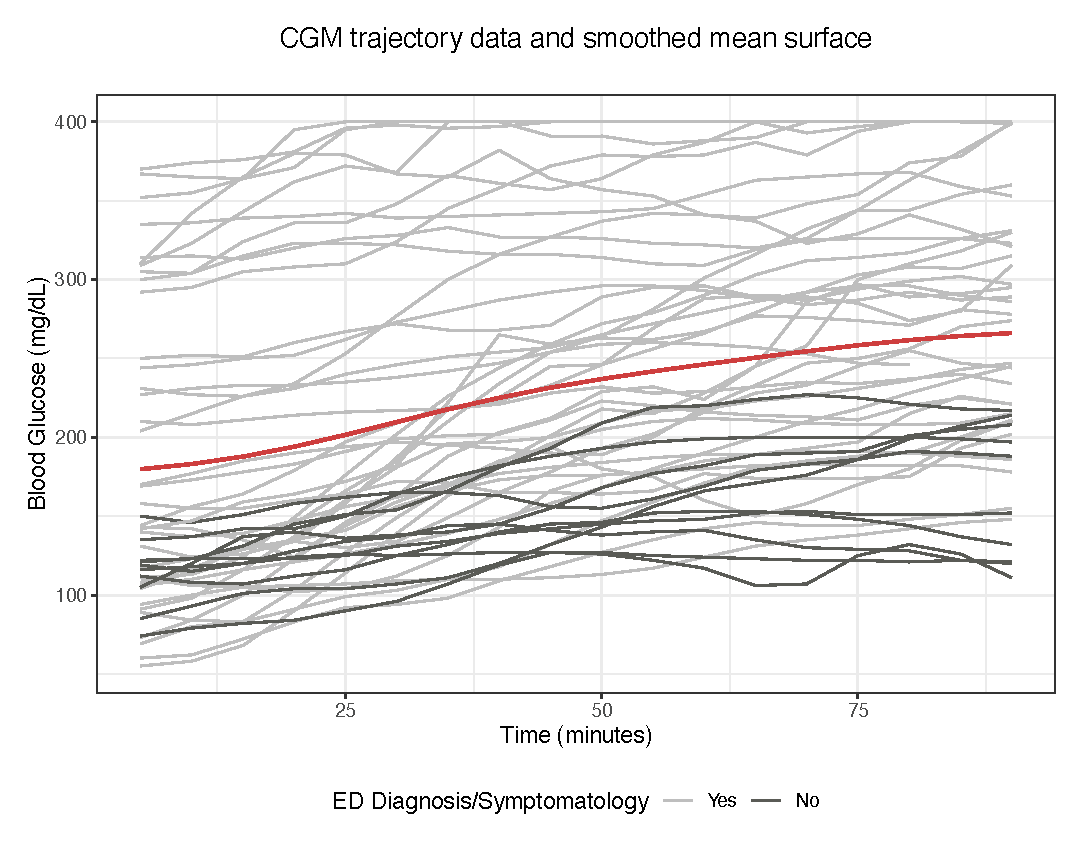
\includegraphics[width=0.5\textwidth]{figures/muhat1.eps}}
  \hspace*{\fill}
  {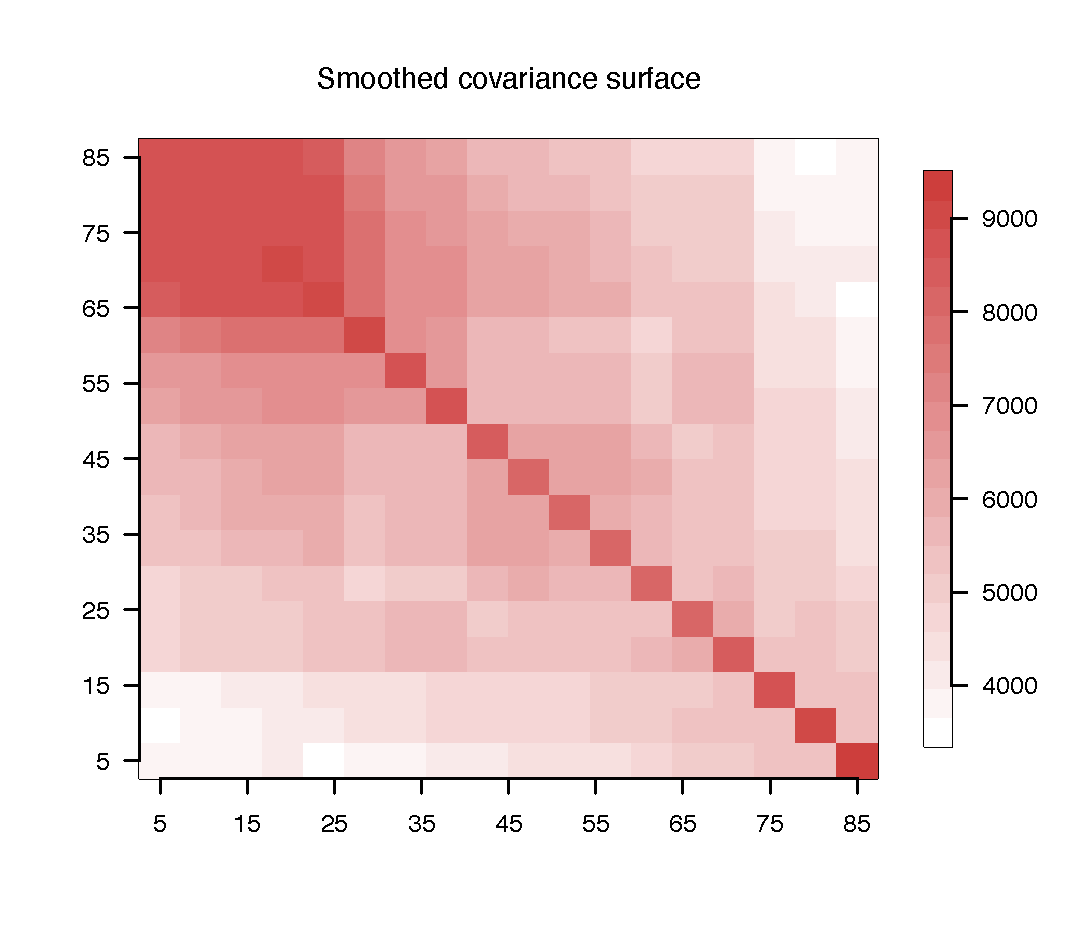
\includegraphics[width=0.47\textwidth]{figures/Sigmahat1.eps}}
  \caption{Left: Blood glucose trajectories from the training data (grey) with the estimated mean function (red) overlayed. Right: Estimated covariance surface.}\label{fig:fig1}
\end{figure}


\section*{Equations}
\begin{itemize}
\item Use \texttt{\textbackslash widehat\{ \}} and \texttt{\textbackslash widetilde\{ \}} instead of
\texttt{\textbackslash hat\{ \}} and \texttt{\textbackslash tilde\{ \}}. The difference is $\widehat{\Sigma}$ versus $\hat{\Sigma}$.
\item Use \texttt{\textbackslash left} and \texttt{\textbackslash right} around parentheses brackets, etc. in displayed equations. For example,
\begin{align}
&(\sum_{i=1}^n x_i^2)^{1/2}\label{eq:normal}\\
&\left (\sum_{i=1}^n x_i^2 \right )^{1/2}\label{eq:rightleft},
\end{align}
where equation \ref{eq:normal} uses normal parentheses and equation \ref{eq:rightleft} uses \texttt{\textbackslash left (} and \texttt{\textbackslash right )}.
\item Theorems can be displayed using the \texttt{theorem} environment. For example:
\begin{theorem}
Theorem details...
\end{theorem}
\end{itemize}




\newpage
\bibliographystyle{biom}
\bibliography{paper-ref}



\label{lastpage}
\end{document}